% Options for packages loaded elsewhere
\PassOptionsToPackage{unicode}{hyperref}
\PassOptionsToPackage{hyphens}{url}
\PassOptionsToPackage{dvipsnames,svgnames,x11names}{xcolor}
%
\documentclass[
  number]{elsarticle}

\usepackage{amsmath,amssymb}
\usepackage{iftex}
\ifPDFTeX
  \usepackage[T1]{fontenc}
  \usepackage[utf8]{inputenc}
  \usepackage{textcomp} % provide euro and other symbols
\else % if luatex or xetex
  \usepackage{unicode-math}
  \defaultfontfeatures{Scale=MatchLowercase}
  \defaultfontfeatures[\rmfamily]{Ligatures=TeX,Scale=1}
\fi
\usepackage{lmodern}
\ifPDFTeX\else  
    % xetex/luatex font selection
\fi
% Use upquote if available, for straight quotes in verbatim environments
\IfFileExists{upquote.sty}{\usepackage{upquote}}{}
\IfFileExists{microtype.sty}{% use microtype if available
  \usepackage[]{microtype}
  \UseMicrotypeSet[protrusion]{basicmath} % disable protrusion for tt fonts
}{}
\makeatletter
\@ifundefined{KOMAClassName}{% if non-KOMA class
  \IfFileExists{parskip.sty}{%
    \usepackage{parskip}
  }{% else
    \setlength{\parindent}{0pt}
    \setlength{\parskip}{6pt plus 2pt minus 1pt}}
}{% if KOMA class
  \KOMAoptions{parskip=half}}
\makeatother
\usepackage{xcolor}
\setlength{\emergencystretch}{3em} % prevent overfull lines
\setcounter{secnumdepth}{5}
% Make \paragraph and \subparagraph free-standing
\makeatletter
\ifx\paragraph\undefined\else
  \let\oldparagraph\paragraph
  \renewcommand{\paragraph}{
    \@ifstar
      \xxxParagraphStar
      \xxxParagraphNoStar
  }
  \newcommand{\xxxParagraphStar}[1]{\oldparagraph*{#1}\mbox{}}
  \newcommand{\xxxParagraphNoStar}[1]{\oldparagraph{#1}\mbox{}}
\fi
\ifx\subparagraph\undefined\else
  \let\oldsubparagraph\subparagraph
  \renewcommand{\subparagraph}{
    \@ifstar
      \xxxSubParagraphStar
      \xxxSubParagraphNoStar
  }
  \newcommand{\xxxSubParagraphStar}[1]{\oldsubparagraph*{#1}\mbox{}}
  \newcommand{\xxxSubParagraphNoStar}[1]{\oldsubparagraph{#1}\mbox{}}
\fi
\makeatother


\providecommand{\tightlist}{%
  \setlength{\itemsep}{0pt}\setlength{\parskip}{0pt}}\usepackage{longtable,booktabs,array}
\usepackage{calc} % for calculating minipage widths
% Correct order of tables after \paragraph or \subparagraph
\usepackage{etoolbox}
\makeatletter
\patchcmd\longtable{\par}{\if@noskipsec\mbox{}\fi\par}{}{}
\makeatother
% Allow footnotes in longtable head/foot
\IfFileExists{footnotehyper.sty}{\usepackage{footnotehyper}}{\usepackage{footnote}}
\makesavenoteenv{longtable}
\usepackage{graphicx}
\makeatletter
\def\maxwidth{\ifdim\Gin@nat@width>\linewidth\linewidth\else\Gin@nat@width\fi}
\def\maxheight{\ifdim\Gin@nat@height>\textheight\textheight\else\Gin@nat@height\fi}
\makeatother
% Scale images if necessary, so that they will not overflow the page
% margins by default, and it is still possible to overwrite the defaults
% using explicit options in \includegraphics[width, height, ...]{}
\setkeys{Gin}{width=\maxwidth,height=\maxheight,keepaspectratio}
% Set default figure placement to htbp
\makeatletter
\def\fps@figure{htbp}
\makeatother

\makeatletter
\@ifpackageloaded{caption}{}{\usepackage{caption}}
\AtBeginDocument{%
\ifdefined\contentsname
  \renewcommand*\contentsname{Table of contents}
\else
  \newcommand\contentsname{Table of contents}
\fi
\ifdefined\listfigurename
  \renewcommand*\listfigurename{List of Figures}
\else
  \newcommand\listfigurename{List of Figures}
\fi
\ifdefined\listtablename
  \renewcommand*\listtablename{List of Tables}
\else
  \newcommand\listtablename{List of Tables}
\fi
\ifdefined\figurename
  \renewcommand*\figurename{Figure}
\else
  \newcommand\figurename{Figure}
\fi
\ifdefined\tablename
  \renewcommand*\tablename{Table}
\else
  \newcommand\tablename{Table}
\fi
}
\@ifpackageloaded{float}{}{\usepackage{float}}
\floatstyle{ruled}
\@ifundefined{c@chapter}{\newfloat{codelisting}{h}{lop}}{\newfloat{codelisting}{h}{lop}[chapter]}
\floatname{codelisting}{Listing}
\newcommand*\listoflistings{\listof{codelisting}{List of Listings}}
\makeatother
\makeatletter
\makeatother
\makeatletter
\@ifpackageloaded{caption}{}{\usepackage{caption}}
\@ifpackageloaded{subcaption}{}{\usepackage{subcaption}}
\makeatother

\ifLuaTeX
  \usepackage{selnolig}  % disable illegal ligatures
\fi
\usepackage[]{natbib}
\bibliographystyle{elsarticle-num}
\usepackage{bookmark}

\IfFileExists{xurl.sty}{\usepackage{xurl}}{} % add URL line breaks if available
\urlstyle{same} % disable monospaced font for URLs
\hypersetup{
  pdftitle={Economic Complexity of Australian Regions},
  pdfauthor={Hamish Gamble; Sharif Rasel},
  pdfkeywords={Economic Complexity, Advanced Manufacturing},
  colorlinks=true,
  linkcolor={blue},
  filecolor={Maroon},
  citecolor={Blue},
  urlcolor={Blue},
  pdfcreator={LaTeX via pandoc}}


\setlength{\parindent}{6pt}
\begin{document}

\begin{frontmatter}
\title{Economic Complexity of Australian Regions}
\author[1]{Hamish Gamble%
\corref{cor1}%
}
 \ead{hamish.gamble@flinders.edu.au} 
\author[1]{Sharif Rasel%
%
}


\affiliation[1]{organization={Flinders University},,postcodesep={}}

\cortext[cor1]{Corresponding author}


        





\begin{keyword}
    Economic Complexity \sep 
    Advanced Manufacturing
\end{keyword}
\end{frontmatter}
    

\subsection{Introduction}\label{introduction}

\subsection{Literature Review}\label{literature-review}

\citep{hidalgo2009} introduced the concept of economic complexity as a
means of quantifying and explaining differences in the economic
development trajectory of different countries. Their method used
bilateral trade data to identify the network structure of countries and
the products they export and built on the concept of relatedness
introduced in \citep{hidalgo2007}. Economic complexity has been shown to
be predictor of

Relatedness has since been applied across industry \citep{neffke2012},
research areas \citep{guevara2016}, occupation \citep{muneepeerakul2013}
and technology (patents) \citep{kogler2013}.

The relatedness approach has also been used to quantify economic
complexity across cities, states, and regions, using employment
data{[}\citep{ecus}; @ecnz; \citep{ecmexico}{]}, business
counts\citep{ecchina}, patent classifications \citep{balland2021}, and
interstate and international trade data \citep{ecaus}.

Despite differences in data sources, the method for calculating economic
complexity in the literature is relatively standard. The presence of an
activity in a region is often identified using a location quotient
method, such that an activity is said to be present in a region if:

\[\frac{X_a^r/\sum_{a}X_a^r}{\sum_{r}X_a^r/\sum_{r,a}X_a^r} \geq 1\]

Where \(X\) is the measure of an activity \(a\) in region \(r\) - such
as the level of employment in an occupation in a city, or the number of
businesses classified in an industry in a province, or the value of
exports of a product from a country. The location quotient method
creates a binary matrix \(M\) with \(a\) rows and \(r\) columns.

\begin{itemize}
\tightlist
\item
  In a study of the economic complexity of US regions, \citep{ecus} use
  metropolitan areas as the basis for calculations.
\item
  Metropolitan areas in the United States are defined such that jobs
  within a given area are held by residents who live in that area.
\item
  Metropolitan areas have a population of at least 50,000 people. The
  smallest MSA was estimated to have a 2023 population of 57,700 (about
  0.015\% of US population).
\item
\end{itemize}

\subsubsection{Small (n) areas}\label{small-n-areas}

\begin{itemize}
\item
  In New Zealand, \citep{ecnz} use weighted correlations of local
  employment shares. Regions range from a population of 1,434 to 573,150
  with a mean population of 29,947 and median population of 6,952.
  Employment is measured as an industry-occupation pair.
\item
  \citep{hidalgo2007} and others have focused on the co-occurrence of
  revealed comparative advantage indices, derived from a location
  quotient. The location quotient is measured as:

  \[
  LQ = \frac{X_r^a/X_r}{X^a/X}
  \]
\item
  As such, small values of \(\frac{X^a}{X}\) can exacerbate any
  measurement error in the numerator. Additionally, the binary nature of
  measuring revealed comparative advantage when the location quotient is
  greater than 1, results in a discontinuity at \(LQ = 1\).
\item
  Differences in relationship between complexity and relatedness on
  indicators may be entirely context dependent.
\end{itemize}

\subsection{Data \& Methods}\label{sec-data-methods}

\subsubsection{Data}\label{data}

\begin{itemize}
\item
  Calculate economic complexity indicators for Australian regions using
  employment data from the 2021 Census.
\item
  Regions classified by Statistical Areas Level 3 (SA3)
\item
  Economic activity classified by ANZSIC industry division and ANZSCO
  major group
\end{itemize}

\textsubscript{Source:
\href{https://aiti-flinders.github.io/sirp-complexity/index.qmd.html}{Article
Notebook}}

\begin{itemize}
\item
  We exclude individuals who identify their place of work as a Migratory
  - Offshore - Shipping region or as No Fixed Address. Employment in
  these regions totals 497,913 or about 4\% of the total sample.
\item
  Following \citep{ecnz}, employment is aggregated into
  industry-occupation pairs, allowing for differentiation between, for
  example, managers working in agriculture, forestry, and fishing, and
  managers working in retail trade.
\item
  Dataset covers 340 regions and 152 industry-occupations.
  Figure~\ref{fig-employment-density} shows the presence of any level of
  employment within a region and industry-occupation. As can be seen,
  there is a high level of employment density across our data.
\end{itemize}

\phantomsection\label{cell-fig-employment-density}
\begin{figure}[H]

\centering{

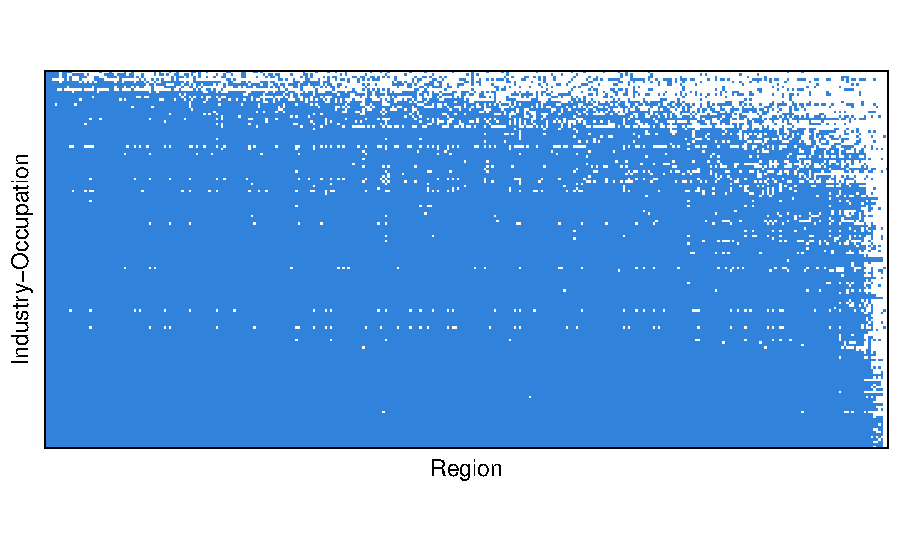
\includegraphics{index_files/figure-pdf/fig-employment-density-1.pdf}

}

\caption{\label{fig-employment-density}Presence of employment across
regions and industry-occupations.}

\end{figure}%

\textsubscript{Source:
\href{https://aiti-flinders.github.io/sirp-complexity/index.qmd.html}{Article
Notebook}}

\subsubsection{Method}\label{method}

This section follows the method of \citep{ecnz} using correlations of
employment shares rather than a location quotient method.

\paragraph{Relatedness}\label{relatedness}

Activities are related based on the weighted correlation between the
local activity share of employment, weighted by each regions share of
total employment.

\begin{itemize}
\tightlist
\item
  First calculate the weighted covariance
\end{itemize}

\[
cov_{aa} = \sum_{c \in C} (\frac{E_c^{a_i}}{E_c}-\frac{E^{a_i}}{E})(\frac{E_c^{a_j}}{E_c}-\frac{E^{a_j}}{E})
\]

\begin{itemize}
\item
  Divide the weighted covariance by the city share-weighted standard
  deviations of the local activity shares to get the weighted
  correlation.
\item
  Map the correlation to the interval \([0,1]\) such that:

  \[
  r_{aa} = \frac{1}{2}(cor(a_i, a_j) + 1)
  \]
\end{itemize}

City relatedness is calculated symmetrically such that:

\[
r_{cc} = \frac{1}{2}(cor(c_i, c_j) + 1)
\]

\paragraph{Complexity}\label{complexity}

Activity complexity is defined by the second eigenvector of the matrix
\(r_{aa}\) and city complexity is defined by the second eigenvector of
the matrix \(r_{cc}\). The sign of activity complexity is set such that
it is positively correlated with the weighted mean size of cities that
contain activity \(a\), and the sign of city complexity is set such that
it is positively correlated with the local share-weighted mean
complexity of activities in city \(c\)

\textsubscript{Source:
\href{https://aiti-flinders.github.io/sirp-complexity/index.qmd.html}{Article
Notebook}}

\subsection{Results}\label{results}

\textsubscript{Source:
\href{https://aiti-flinders.github.io/sirp-complexity/index.qmd.html}{Article
Notebook}}

Figure~\ref{fig-gcc-complexity} shows the regional complexity of SA3
regions in Australian Greater Capital City Areas based on 2021 Census
data. Complexity is highest in capital cities and surrounding regions.

\phantomsection\label{cell-fig-gcc-complexity}
\begin{figure}[H]

\centering{

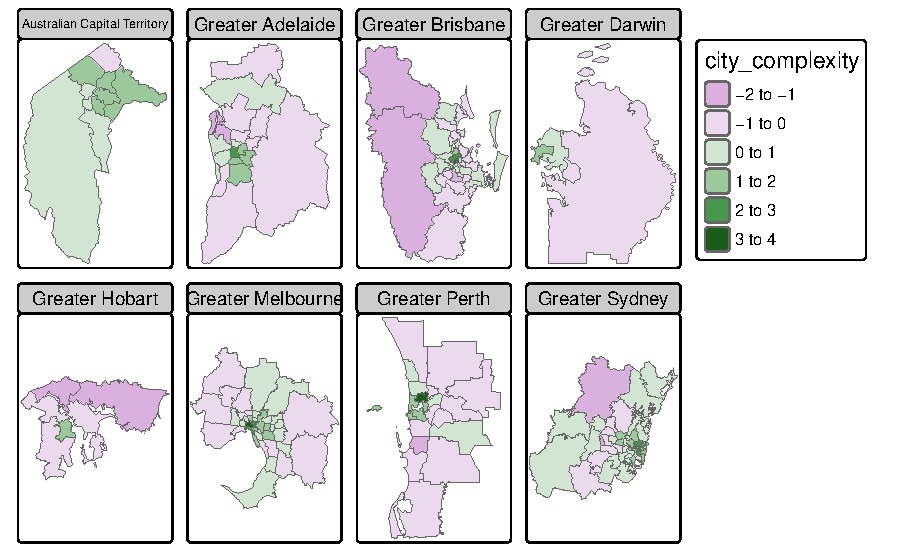
\includegraphics{index_files/figure-pdf/fig-gcc-complexity-1.pdf}

}

\caption{\label{fig-gcc-complexity}Complexity of Australian Greater
Capital City Areas}

\end{figure}%

\textsubscript{Source:
\href{https://aiti-flinders.github.io/sirp-complexity/index.qmd.html}{Article
Notebook}}

\subsubsection{Spatial Correlation}\label{spatial-correlation}

\begin{itemize}
\tightlist
\item
  Is economic complexity correlated across space?
\end{itemize}

\textsubscript{Source:
\href{https://aiti-flinders.github.io/sirp-complexity/index.qmd.html}{Article
Notebook}}

\begin{itemize}
\tightlist
\item
  Global Moran's I = 0.5007756 with a p.value of 0.
\end{itemize}

\phantomsection\label{cell-fig-complexity-hot-spots}
\begin{figure}[H]

\centering{

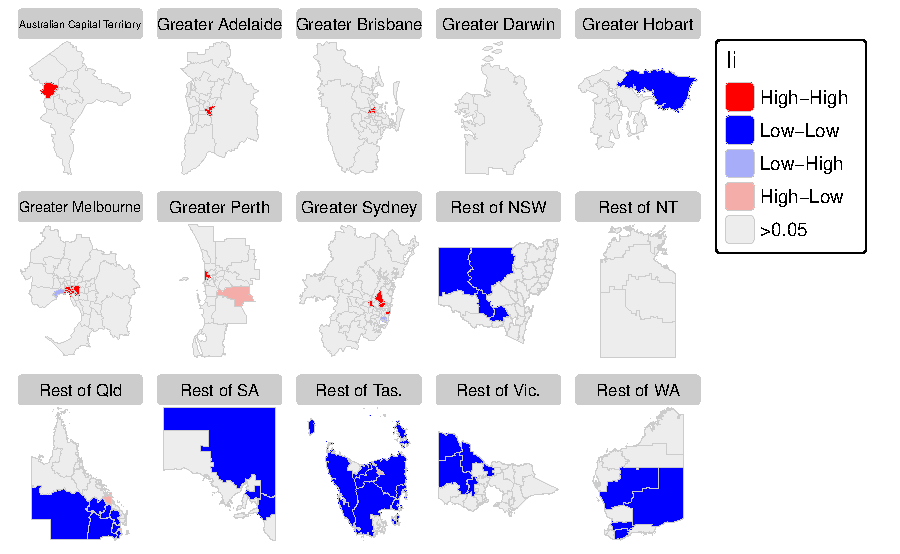
\includegraphics{index_files/figure-pdf/fig-complexity-hot-spots-1.pdf}

}

\caption{\label{fig-complexity-hot-spots}City Complexity hot spots
(based on local Moran's I p.values)}

\end{figure}%

\textsubscript{Source:
\href{https://aiti-flinders.github.io/sirp-complexity/index.qmd.html}{Article
Notebook}}

\subsection{Conclusion}\label{conclusion}

\subsection*{References}\label{references}
\addcontentsline{toc}{subsection}{References}

\renewcommand{\bibsection}{}
\bibliography{references.bib}





\end{document}
